%
% komplex.tex -- komplexe Zahlen
%
% (c) 2021 Prof Dr Andreas Müller, OST Ostschweizer Fachhochschule
%
\section{Komplexe Zahlen
\label{buch:section:komplexe-zahlen}}
\rhead{Komplexe Zahlen}
In den reellen Zahlen lassen sich viele algebraische Gleichungen lösen,
die in $\mathbb{Q}$ nicht lösbar waren.
Andere, z.~B.~die Gleichung
\begin{equation}
x^2+1=0,
\label{buch:zahlen:eqn:igleichung}
\end{equation}
haben weiterhin keine Lösung.
Der Grund dafür ist das Bestreben bei der Konstruktion der reellen Zahlen, 
die Ordnungsrelation zu erhalten.
\index{Ordnungsrelation}%
Diese ermöglicht, Näherungsintervalle und Intervallschachtelungen
zu definieren.

Die Ordnungsrelation sagt aber auch, dass $x^2\ge 0$ ist für jedes
$x\in\mathbb{R}$, so dass $x^2+1>0$ sein muss.
Dies ist der Grund, warum die Gleichung \ref{buch:zahlen:eqn:igleichung}
keine Lösung in $\mathbb{R}$ haben kann.
Im Umkehrschluss folgt auch, dass eine Erweiterung der reellen Zahlen,
in der die Gleichung \eqref{buch:zahlen:eqn:igleichung} lösbar ist,
ohne die Ordnungsrelation auskommen muss.
Es muss darin Zahlen geben, deren Quadrat negativ ist und der
Grössenvergleich dieser Zahlen untereinander ist nur eingeschränkt
möglich.

\subsubsection{Imaginäre und komplexe Zahlen}
Den reellen Zahlen fehlen also Zahlen, deren Quadrat negativ ist.
Nach inzwischen bewährtem Muster konstruieren wird die neuen Zahlen
daher als Paare $(a,b)$.
Die erste Komponente soll die bekannten reellen Zahlen darstellen,
deren Quadrat positiv ist.
Die zweite Komponente soll für die Zahlen verwendet werden, deren Quadrat
negativ ist.
Die Zahl, deren Quadrat $-1$ sein soll, bezeichnen wir mit dem
Paar $(0,1)$ und schreiben dafür auch $i=(0,1)$ mit $i^2=-1$.
Das Paar $i=(0,1)$ heisst auch die {\em imaginäre Einheit}.
\index{imaginäre Einheit}%

Die Rechenregeln sollen weiterhin erhalten bleiben, sie müssen daher
wie folgt definiert werden:
\begin{equation}
\begin{aligned}
(a,b) + (c,d) &= (a+c,b+d) &&& (a+bi) + (c+di) &= (a+c) + (b+d)i
\\
(a,b) \cdot (c,d) &= (ad-bd, ad+bc) &&& (a+bi)\cdot(c+di) &= ac-bd + (ad+bc)i.
\end{aligned}
\label{buch:zahlen:cregeln}
\end{equation}
Diese Regeln ergeben sich ganz natürlich aus den Rechenregeln
in $\mathbb{R}$ unter Berücksichtigung der Regel $i^2=-1$.

Eine komplexe Zahl ist ein solches Paar, die Menge der komplexen Zahlen
ist
\[
\mathbb{C}
=
\{a+bi\;|\;a,b\in\mathbb{R}\}
\]
mit den Rechenoperationen~\eqref{buch:zahlen:cregeln}.
Die Menge $\mathbb{C}$ verhält sich daher wie eine zweidimensionaler
reeller Vektorraum mit Basisvektoren $1$ und $i$.

\subsubsection{Real- und Imaginärteil}
Ist $z=a+bi$ eine komplexe Zahl, dann heisst $a$ der {\em Realteil} $a=\Re z$
\index{Realteil}%
und $b$ heisst der {\em Imaginärteil} $\Im z$.
\index{Imaginärteil}%
Real- und Imaginärteil sind lineare Abbildungen $\mathbb{C}\to\mathbb{R}$,
wenn man $\mathbb{C}$ als linearen $\mathbb{R}$-Vektorraum betrachtet.
Sie projizieren einen Punkt auf die Koordinatenachsen, die entsprechend
auch die {\em reelle} und die {\em imaginäre Achse} heissen.
\index{reelle Achse}%
\index{imaginäre Achse}%

Die Multiplikation mit $i$ vertauscht Real- und Imaginärteil:
\[
\Re (iz)
=
-b
=
-\Im z
\qquad\text{und}\qquad
\Im (iz)
=
a
=
\Re z.
\]
Zusätzlich kehrt das Vorzeichen der einen Komponente.
Wir kommen auf diese Eigenschaft zurück, wenn wir später in
Abschnitt~\ref{buch:grundlagen:subsection:ringe}
komplexe Zahlen als Matrizen beschreiben.

\subsubsection{Gausssche Zahlenebene}
Beschränkt man die Multiplikation auf einen reellen Faktor, wird $\mathbb{C}$,
wie wir bereits ausgeführt haben,
zu einem zweidimensionalen reellen Vektorraum.
Man kann die komplexe Zahl $a+bi$ daher auch als Punkt $(a,b)$ in der
sogenannten {\em Gaussschen Ebene} betrachten (Abbildung~\ref{buch:zahlen:cfig}).
\index{Gaussche Zahlenebene}%
Die Addition von komplexen Zahlen ist in diesem Bild die vektorielle
Addition, die Multiplikation mit reellen Zahlen werden wir weiter unten
genauer untersuchen müssen.

\begin{figure}
\centering
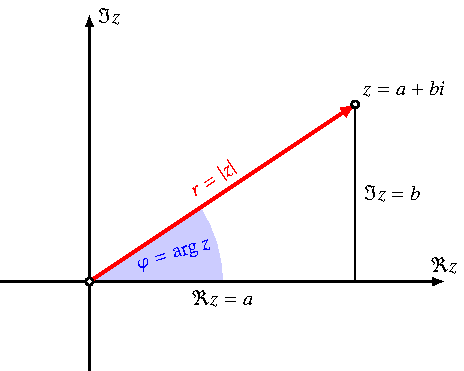
\includegraphics{chapters/05-zahlen/images/komplex.pdf}
\caption{Argument und Betrag einer komplexen Zahl $z=a+ib$ in der 
Gaussschen Zahlen\-ebene
\label{buch:zahlen:cfig}}
\end{figure}%

Die Zahlenebene führt auf eine weitere mögliche Parametrisierung einer
komplexen Zahl.
Ein Punkt $z$ der Ebene kann in Polarkoordinaten auch durch den {\em Betrag}
\index{Betrag}%
\index{Polarkoordinaten}%
und den Winkel zwischen der reellen Achse und dem Radiusvektor zum Punkt,
dem sogenannten {\em Argument},
charakterisiert werden.

\subsubsection{Komplexe Konjugation}
Der komplexen Zahl $u=a+bi$ ordnen wir die sogenannte
{\em komplex konjugierte} Zahl $\overline{z} = a-bi$ zu.
Mit Hilfe der komplexen Konjugation $z\mapsto\overline{z}$
kann man den Real- und Imaginärteil
\index{komplexe Konjugation}%
\index{Konjugation, komplexe}%
algebraisch ausdrücken:
\[
\Re z 
=
\frac{z+\overline{z}}2
=
\frac{a+bi+a-bi}{2}
=
\frac{2a}2
=a
\qquad\text{und}\qquad
\Im z
=
\frac{z-\overline{z}}{2i}
=
\frac{a+bi-a+bi}{2i}
=
\frac{2bi}{2i}
=
b.
\]
In der Gaussschen Zahlenebene ist die komplexe Konjugation eine
Spiegelung an der reellen Achse.

\subsubsection{Betrag}
In $\mathbb{R}$ kann man die Ordnungsrelation dazu verwenden zu entscheiden,
ob eine Zahl $0$ ist. 
Wenn $x\ge 0$ ist und $x\le 0$, dann ist $x=0$.
In $\mathbb{C}$ steht diese Ordnungsrelation nicht mehr zur Verfügung.
Eine komplexe Zahl ist von $0$ verschieden, wenn die Länge des Vektors in der
Zahlenebene verschieden von $0$ ist.
Wir definieren daher den {\em Betrag} einer komplexen Zahl $z=a+bi$ als
\index{Betrag}
\[
|z|^2
=
a^2 +b^2
=
(\Re z)^2 + (\Im z)^2
\qquad\Rightarrow\qquad
|z|
=
\sqrt{a^2+b^2}
=
\sqrt{(\Re z)^2 + (\Im z)^2}.
\]
Der Betrag lässt sich auch mit Hilfe der komplexen Konjugation ausdrücken,
es ist $z\overline{z} = (a+bi)(a-bi) = a^2+abi-abi+b^2 = |z|^2$.
Der Betrag ist immer eine reelle Zahl.

\subsubsection{Division}
Die Erweiterung zu den komplexen Zahlen muss auch die Division erhalten.
Dies ist durchaus nicht selbstverständlich.
Man kann zeigen, dass ein Produkt von Vektoren eines Vektorraums nur für
einige wenige, niedrige Dimensionen überhaupt möglich ist.
Für die Division sind die Einschränkungen noch gravierender, die einzigen
Dimensionen $>1$, in denen ein Produkt mit einer Division definiert werden
kann\footnote{Der Beweis dieser Aussage ist ziemlich schwierig und wurde
erst im 20.~Jahrhundert mit Hilfe der Methoden der algebraischen Topologie
erbracht. Eine Übersicht über den Beweis kann in Kapitel~10 von
\cite{buch:ebbinghaus} gefunden werden.}, sind $2$, $4$ und $8$.
Nur in Dimension $2$ ist ein kommutatives Produkt möglich, dies muss das
Produkt der komplexen Zahlen sein.

Wie berechnet man den Quotienten $\frac{z}{w}$ für zwei beliebige komplexe
Zahlen $z=a+bi$ und $w=c+di$ mit $w\ne 0$?
Dazu erweitert man den Bruch mit der komplex Konjugierten des Nenners:
\begin{align*}
\frac{z}{w}
&=
\frac{z\overline{w}}{w\overline{w}}
=
\frac{z\overline{w}}{|w|^2}
\end{align*}
Da der Nenner $|w|^2>0$ eine reelle Zahl ist, ist die Division einfach,
es ist die Multiplikation mit der reellen Zahl $1/|w|^2$.

Wir können den Quotienten auch durch Real- und Imaginärteil ausdrücken:
\begin{align*}
\frac{z}{w}
&=
\frac{a+bi}{c+di}
=
\frac{(a+bi)(c+di)}{(c+di)(c-di)}
=
\frac{ac-bd +(ad+bc)i}{c^2+d^2}.
\end{align*}


\subsubsection{Geometrische Interpretation der Rechenoperationen}
Die Addition komplexer Zahlen wurde bereits als Vektoraddition
in der Gausschen Zahlenebene interpretiert. 
Die Multiplikation ist etwas komplizierter, wir berechnen Betrag
und Argument von $zw$ separat.
Für den Betrag erhalten wir
\begin{align*}
|zw|^2
&=
zw\overline{(zw)}
=
zw\overline{z}\overline{w}
=
z\overline{z}w\overline{w}
=
|z|^2|w|^2
\end{align*}
Der Betrag des Produktes ist also das Produkt der Beträge.

Für das Argument verwenden wir, dass
\[
\tan\operatorname{arg}z
=
\frac{\Im z}{\Re z}
=
\frac{b}{a}
\qquad\Rightarrow\qquad
b=a\tan\operatorname{arg}z
\]
und analog für $w$.
Bei der Berechnung des Produktes behandeln wir nur den Fall $a\ne 0$ 
und $c\ne 0$, was uns ermöglicht, den Bruch durch $ac$ zu kürzen:
\begin{align*}
\tan\arg wz
&=
\frac{\Im wz}{\Re wz}
=
\frac{ad+bc}{ac-bd}
=
\frac{\frac{d}{c} + \frac{b}{a}}{1-\frac{b}{a}\frac{d}{c}}
=
\frac{
\tan\operatorname{arg}z+\tan\operatorname{arg}w
}{
1+
\tan\operatorname{arg}z\cdot\tan\operatorname{arg}w
}
=
\tan\bigl(
\operatorname{arg}z+\operatorname{arg}w
\bigr).
\end{align*}
Im letzten Schritt haben wir die Additionsformel für den Tangens verwendet.
\index{Additionstheorem für Tangens}%
Daraus liest man ab, dass das Argument eines Produkts die Summe der
Argumente ist.
Die Multiplikation mit einer festen komplexen Zahl führt also mit der ganzen
komplexen Ebene eine Drehstreckung durch.
Auf diese geometrische Beschreibung der Multiplikation werden wir zurückkommen,
wenn wir die komplexen Zahlen als Matrizen beschreiben wollen.

\subsubsection{Algebraische Vollständigkeit}
Die komplexen Zahlen $\mathbb{C}$ sind als Erweiterung von $\mathbb{R}$
so konstruiert worden, dass die Gleichung $x^2+1=0$ eine Lösung hat.
Etwas überraschend ist dagegen, dass in dieser Erweiterung jetzt jede
beliebige algebraische Gleichung lösbar geworden ist.
Dies ist der Inhalt des Fundamentalsatzes der Algebra.

\begin{satz}[Fundamentalsatz der Algebra]
\label{buch:zahlen:satz:fundamentalsatz}
\index{Fundamentalsatz der Algebra}%
Jede algebraische Gleichung der Form
\[
p(x)=x^n + a_{n-1}x^{n-1}+a_1x+a_0=0,\qquad a_k\in\mathbb{C}
\]
mit komplexen Koeffizienten hat $n$ möglicherweise mit Vielfachheit
gezählte Nullstellen $\alpha_1,\dots,\alpha_m$, d.~h.~das Polynom $p(x)$
lässt sich in Linearfaktoren
\[
p(x)
=
(x-\alpha_1)^{k_1}(x-\alpha_2)^{k_2}\cdot\ldots\cdot(x-\alpha_m)^{k_m}
\]
zerlegen, wobei $k_1+k_2+\dots+k_m=n$.
Die Zahl $k_j$ heisst die {\em Vielfachheit} der Nullstelle $\alpha_j$.
\end{satz}

Der Fundamentalsatz der Algebra wurde erstmals von Carl Friedrich Gauss
\index{Gauss, Carl Friedrich}%
vollständig bewiesen.
Seither sind viele alternative Beweise mit Methoden aus den verschiedensten
Gebieten der Mathematik gegeben worden.
Etwas salopp könnten man sagen, dass der Fundamentalsatz ausdrückt, dass
die Konstruktion der Zahlensysteme mit $\mathbb{C}$ abgeschlossen ist,
soweit damit die Lösbarkeit beliebiger Gleichungen angestrebt ist.

\subsubsection{Quaternionen und Octonionen}
Die komplexen Zahlen ermöglichen eine sehr effiziente Beschreibung 
geometrischer Abbildungen wie Translationen, Spiegelungen und 
Drehstreckungen in der Ebene.
Es drängt sich damit die Frage auf, ob sich $\mathbb{C}$ so erweitern
lässt, dass man damit auch Drehungen im dreidimensionalen Raum
beschreiben könnte.
Da Drehungen um verschiedene Achsen nicht vertauschen, kann eine solche
Erweiterung nicht mehr kommutativ sein.

William Rowan Hamilton propagierte ab 1843 eine Erweiterung von $\mathbb{C}$
\index{Hamilton, William Rowan}%
mit zwei zusätzlichen Einheiten $j$ und $k$ mit den nichtkommutativen
Relationen
\begin{equation}
i^2 = j^2 = k^2 = i\!jk = -1.
\label{buch:zahlen:eqn:quaternionenregeln}
\end{equation}
Er nannte die Menge aller Linearkombinationen 
\[
\mathbb{H} = \{ a_0+a_1i+a_2j+a_3k\;|\; a_l\in \mathbb{R}\}
\]
die {\em Quaternionen}, die Einheiten $i$, $j$ und $k$ heissen auch
\index{Quaternionen}%
Einheitsquaternionen.
\index{Einheitsquaternionen}%
Konjugation, Betrag und Division können ganz ähnlich wie bei den
\index{Konjugation von Quaternionen}%
\index{Betrag einer Quaternion}%
\index{Division durch eine Quaternion}%
komplexen Zahlen definiert werden und machen $\mathbb{H}$ zu einer
sogenannten {\em Divisionsalgebra}.
\index{Divisionsalgebra}%
Alle Rechenregeln mit Ausnahme der Kommutativität der Multiplikation
sind weiterhin gültig und durch jede von $0$ verschiedene Quaternion
kann auch dividiert werden.

Aus den Regeln für die Quadrate der Einheiten in
\eqref{buch:zahlen:eqn:quaternionenregeln} folgt zum Beispiel
$i^{-1}=-i$, $j^{-1}=-j$ und $k^{-1}=-k$.
Die letzte Bedingung liefert daraus
\[
i\!jk=-1
\qquad\Rightarrow\qquad
\left\{
\quad
\begin{aligned}
i\!j
&=
i\!jkk^{-1}=-1k^{-1}=k
\\
i^2\!jk&=-i=-jk
\\
-j^2k&=-ji=k
\end{aligned}
\right.
\]
Aus den Relationen~\eqref{buch:zahlen:eqn:quaternionenregeln}
folgt also insbesondere auch, dass $i\!j=-ji$.
Ebenso kann abgeleitet werden, dass $jk=-k\!j$ und $ik=-ki$.
Man sagt, die Einheiten sind {\em antikommutativ}.
\index{antikommutativ}%

Die Beschreibung von Drehungen mit Quaternionen ist in der
Computergraphik sehr beliebt, weil eine Quaternion mit nur vier
Komponenten $a_0,\dots,a_3$ vollständig beschrieben ist.
Eine Transformationsmatrix des dreidimensionalen Raumes enthält
dagegen neun Koeffizienten, die vergleichsweise komplizierte 
Abhängigkeiten erfüllen müssen.
Kapitel~\ref{chapter:clifford} behandelt nicht nur die Beschreibung
von Drehungen des dreidimensionalen Raumes sondern eine weitreichende
Verallgemeinerung dieser Idee, die sogenannte {\em geometrische Algebra}.
\index{geometrische Algebra}%
Quaternionen haben auch in weiteren Gebieten interessante Anwendungen,
zum Beispiel in der Quantenmechanik, wo antikommutierende Operatoren
\index{Quantenmechanik}%
bei der Beschreibung von Fermionen eine zentrale Rolle spielen.
\index{Fermion}%

Aus rein algebraischer Sicht kann man die Frage stellen, ob es eventuell
auch noch grössere Divisionsalgebren gibt, die $\mathbb{H}$ erweitern.
Tatsächlich hat Arthur Cayley 1845 eine achtdimensionale Algebra,
die Oktonionen $\mathbb{O}$, mit vier weiteren Einheiten beschrieben.
\index{Cayley, Arthur}%
Allerdings sind die Oktonionen nur beschränkt praktisch anwendbar.
Grund dafür ist die Tatsache, dass die Multiplikation in $\mathbb{O}$
nicht mehr assoziativ ist.
Das Produkt von mehr als zwei Faktoren aus $\mathbb{O}$ ist von der
Reihenfolge der Ausführung der Multiplikationen abhängig.






